 
\section{Litter decomposition and the global carbon cycle}

Rising atmospheric CO$_{2}$ concentrations and global climate changes caused by them \citep{IPCC2007pt1ch1} lead to an increased interest in natural carbon cycles and their anthropogenic modifications. Since pre-industrial times, annual means of athmospheric CO$_{2}$ concentration increased from 280 to 379 ppm (v/v) \citep{IPCC2007pt1ch1}. The source of approximately 80\% of the increase was be pined down to fossil fuel usage by comparing athmospheric CO$_{2}$ concentration to its \textsuperscript{13} C signature (fossil fuel C is depleted in \textsuperscript{13} C ) or corrensponding decrease in athmospheric O$_{2}$ concentrations\citep{IPCC2007pt1ch1}. Furthermore, land use change and cement production are accounted for additional CO$_{2}$ emissions. Between 2000 and 2005, mean annual CO$_{2}$ emissions from fossil fuel burning and cement production accounts for 7.2 $\pm$ 0.3 Gt CO$_{2}$-C. Additionally, land use change causes the annual emmissions 1.6 $\pm$ 1.1 Gt CO$_{2}$-C. Together with other greenhouse gases, elevated CO$_{2}$ concentrations are prognosted to raise earth mean surface temperature by nn degree by 20nn (IPCC?).

Anthropogenic CO$_{2}$ emissions are tightly interconnected with natural carbon cycles. Only 45\% of the emissions are found in the athmosphere, 30\% of the emmited CO$_{2}$ is absorbed in oceans and 25\% in terrestrial ecosystems . Oceanic CO$_{2}$ absorption is based on export of particular and dissolved organic carbon and dissolved inorganic carbon (HCO \textsubscript{3} \textsuperscript{-} , CO \textsubscript{3} \textsuperscript{2-} ) to intermediate and deep water layers. Land sinks take up carbon into larger vegetation- and soil C pools, i.e. due to a nothward shift of climatic limits for vegetation and CO$_{2}$ and N fertilization. However, a large part (-2.6 Gt a\textsuperscript{-1}) of this terrestrial carbon sinks is unaccounted for \citep[p. 515]{IPCC2007pt1ch7}. 

Finding this ``missing sink'' and prognosting feedback mechanisms of CO$_{2}$ emissions challenged scientists to strife for depthening their understanding of large scale biotic carbon transformation processes and storage. Globally, land plants assimilates 120 Gt C annually (gross primary production). This is almost one sixth of the global atmospheric CO$_{2}$ pool (750 Gt a-1) and more than 15 times more than antropogenic C emissions. Autotrophic (plant) respiration consumes one half of the assimilated carbon, the other half is introduced into decomposition process as plant litter. Animal biomass and herbivory form only a neglectable part of the total biomass [lit.], but can wield key controls on vegetation and its succession.

Ecosystem carbon balances are determined by the difference between carbon assimilation (photosynthesis) and respiration. While controls on photosynthesis rates are well understood, knowledge about decomposition processes is by far more limited. This is due to the fact that organisms capable of photosynthesis generally are green, seesile and grow aboveground, are therefore easy to find and study, while a large part of heterotrophic respiration is conducted by soil microbial communities of microscopic scale that dwell belowground, are  hard to identify, and live in a chemically complex environment. Due to the complex nature of soils, studying chemical transformation processes and chemical controls over microbial communities and physiology is easier in aquatic than in terrestrian habitates (for example, differences between nutrient contents and bioavailable nutrient amounts are smaller in aquatic environments, facilitating studies of nutrient control on microbial communities). However, research interest in terrestrial decomposition processes, especially litter decomposition, which sees the highest biomass turnover, is enormous, with more than one peer-reviewed research article per day published on litter decomposition between 2005 and 2009 \citep{Prescott2010}. 

Global litterfall summs up to for approximately 60 Gt C a\textsuperscript{-1}. Frequently between 30 and 70\% of this mass are lost in the first year and further 20 to 30 \% within another 5 to 10 years \citep[p.157]{Chapin2002}.

Temperate forests are highly productive, average net primary production is estimated for 1550 g m\textsuperscript{-2} a\textsuperscript{-1} (1/3 of which is allocated into belowground biomass). They cover 1.7 * 10\textsuperscript{7} km\textsuperscript{2} (~ 1/15th of earth land surface) and account for 8.1 Gt a-1 NPP (1/8th of total terrestrial NPP) \citep[p?]{Chapin2002}. European beech (\emph{Fagus silvaticus} L.) is the dominant tree species in potential western and central Europe. 

\subsection{Ecological stoichiometry}

Carl Sprengel proposed in 1828 that crops rely on nutrints in a given ratio, and that growth is limited by the nutrient that is least frequent compared to this given ratio. While since then plants - and other organisms - were shown to be capeable of a certain plasticity in their nutrient requirement, there is a tradeoff between addaption to nutrient availability and competitive fitness. \footnote{citation}

But organisms do not only rely on elements in a certain ratio, they are also bound (within an adaptive range) to keep them in specific range within their internal mileu. An homeostatic organism keeps this internal mileu constant independent of their ambiental conditions, while in on that is not homeostatic, the internal mileu changes with the elemental ratio in their substrate \citep{Sterner2002}. 

By 1958, marine biologist Albert C. Redford pusblished results from measurements of the elementel composition of marine biomass featuring a constant ratio between carbon, nitrogen, and phosphorous (C:N:P = 106:16:1 (n/n)) in both living and dead biomass. The high constancy of this ratios is based on controls over CO$_2$ assimilation by N and P availability and controls of the  biogeochemical cycling of nutrients (i.e. export by sedimentation) by biological systems \citep{Cleveland2007}. 

Several attempts to find similar ratios in terrestrian ecosystem mostely failed due to the complex nature of terrestrian soils and difficulties to determine actual bioavailability of nutrients. \footnote{paper “redfield ratio for soils” here!}

Plants are able to assimilate carbon from atmosphaeric CO$_2$, but have to sequestrate other elements from soils. Furthermore, a significant part of nitrogen and other nutrients is removed from senecenced leaves before abscission. Therefore, plant detritus is enriched in carbon and depleted in nitrogen when compared to soils or decomposer organisms. C:N ratios (w/w) found in fresh beech litter are between 1:40 and 1:50 \citep{Mooshammer2011}, while soil C:N ratios are in the order of 1:20 \footnote{citation}. Therefore, during litter decomposition, the part of carbon mineralized is higher than the part of nitrogen. Microbial decomposer communities found on early decomposition litter have biomass C:N ratios between 1:6 and 1:18, indicating microbes live in a environment characterized by a carbon surplass and a lack of nitrogen. Litter decomposition rates were found to correlate with detritus C:N and C:P rates \citep{Enriquez1993}.

\section{Chemical constituents of initial beech litter}

The dry biomass of freshly fallen plant litter is chemically dominated by polymeric compounds. Nitrogen is present almost exclusively in for of protein \citep{Wanek2010}, among carbohydrates, cellulose (the $\beta$ - 1-4 glycosidic polymer of glucose) is most common (10-50 \% of litter dry mass). Other carbohydrates - refered to as hemicelluloses - together make up between 30 and 40 \% of litter dry mass. A wide variety of carbohydrate monomeres and glycosidic bindings occur in are leaf litter. Lignin, forms 15-40\% biomass, is an aromatic polymer fromed through the radicalic polymerisation of several different phenylpropanoid monomers. \citep[pp. 54f]{Berg2008}.  The polymerization process of lignin can incorporates protein and carbohydrates into lignin polymers, thereby occluding them to decomposing enzymes and lowering their bioavailability. Nitrogen content of beech lignin was found twice as high as in bulk litter \citep{Dykmans2002}. Furthermore, cutin waxes (ester-bound long chain aliphaic compounds with aromatic components) and tannins are present.

Only a small fraction of foliar plant litter (approximately 25\% for decidous litter, and less in conifer litter) is soluble in water \citep{Berg2008}. Therefore, decomposing microorganisms rely on the excretion of extracellular enzymes to break down plant biomass into soluble fragments \cite{Klotzbucher2011}. Hydrolases break down protein and carbohydrates to amino acids and sugars, while the degradation of lignin is facilitated by oxidoreductases \citep{Sinsabaugh2011}.

\subsection{Micronutrients}

Litter micronutrient content varies and depends in 
Transition metals, especially manganese and iron, are important co-factors of oxidoreductases. The aerobic degradation of complex aromatic compounds is facilitated by reactive oxigen species generated by such enzymes. Therefore, a lack of their cofactors can limit the degradation of complex material (especially phenolic compounds like lignin) in the decomposition processes of litter and other complex organic material like soil orgnic matter or dissolved organic matter. \footnote{references needed!!}

\section{Changes of litter carbon chemistry during decomposition}

\subsection{The traditional model developed by B. Berg}

Traditional models of chemical changes during litter decomposition describe three phases of litter decomposition. In the early phase, which can expand until 40\% of dry mass are lost, availability of labile carbon sources like soluble compounds and non-lignified carbohydrates is high. In this phase, mass loss rate were usually found to be nitrogen limited and - more generally - enhanced by high levels of nitrogen, phosphorous and dissolved carbon. In the late phase, lignin content inhibits further decomposition and mass loss rates are repressed by lignin and nitrogen contents, but enhances by high manganese contents. During this phase, lignin contents reach a constant value. Finally, at the end of decomposition, mass loss of near-humus litter reaches a limit value, and remaining biomass becomes incorporated into soils (fig. \ref{fig:berg}). 

\cite{Berg2008}).

\subsection{Microbial nitrogen mining hypothesis}

The “nitrogen mining hypothesis” is based on the idea, that the breakdown of recalcitrant carbon - while yielding little to no energy - allows soil microbia to access recalcitrant nitrogen. This explains why nitrogen starvation triggers the excretion of enzymes degrading phenolic compounds \citep{Craine2007}. In plant litter, nitrogen is often occluded within lignin molecules, which are degraded by similar enzymes. 


\begin{figure} 
\begin{center} 
%\includegraphics[height=7in,width=5in,angle=90]{file.eps} 
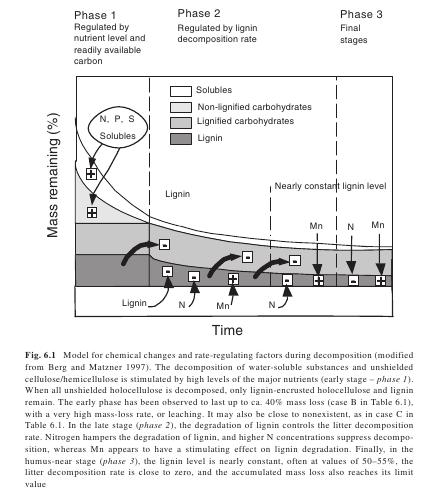
\includegraphics{decompositionmodel_berg.jpg}
\caption{Litter decomposition model (taken from \cite{Berg2008})} 
\label{fig:berg}
\end{center} 
\end{figure}  

\subsection{Carbon limitation of lignin decomposition}

Recently, \cite{Klotzbucher2011} suggested that the degradation of lignin depends on the availability of labile carbon sources. 


\begin{figure} 
\begin{center} 
%\includegraphics[height=7in,width=5in,angle=90]{file.eps} 
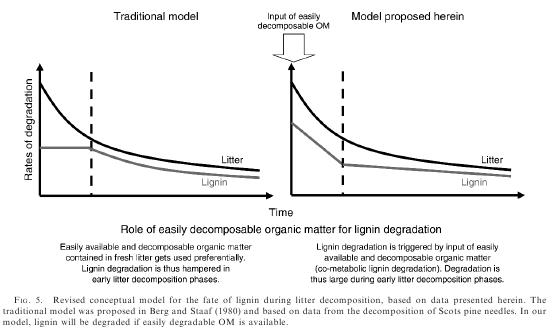
\includegraphics{decompositionmodel_klotzbuecher.jpg}
\caption{Lignin decomposition model (taken from \cite{Klotzbucher2011})} 
\label{fig:klotzbuecher}
\end{center} 
\end{figure}  

\section{Analytical Pyrolysis}

Pyrolysis is the decomposition of complex organic compounds under elevated temperatures in the absence of oxygen. In the case of analytical pyrolysis, Samples are heated to temperatures above 500 \textedegree C in an helium athmosphere, which is later introduced as carrier gas in a GC/MS-system.

%\subsection{Analytical methods to characterize high molecular weight compounds}

%\paragraph{Carbohydrates}
%The characterization of sugar monomers present can be achieved by HPLC or GC analysis after hydrolysis (i.e. \cite{Snajdr2011}). Specific starch analysis is usually conducted by enzymatic hydrolysis with amylases, described by \cite{Leitner2011}. Cellulose and hemicelluloses are  often analyzed by selective extraction and gravimetry. This method is describe in more detail with lignin analysis.

%\paragraph{Lignin}
%Several methods have been developed to determine lignin, but [they are all problematic] \citep{Hatfield2005}.



%section{Anthropogenic disturbances of litter decomposition}

% Litter decomposition controls the release of nutrients and the mineralization of assimilated carbon. 
% 
% Effects of increasiung atmospharic CO$_{2}$ on plants:
% 
% Increasing carboxylation (CO$_{2}$ assimilation) and decreasing oxigenation (O$_{2}$ assimilation). Both effects increase photosynthesis rates. (Farqzhar et al 1980, via IPCC AR4 2007 part 1 p. 195)
% 
% C3 plants generally show an increase in assimilation rates under elevated atmospheric CO$_{2}$ concentrations. C4 plants show no increase or an increase inferior to C3 plants, as they already posses a mechanism to concentrate CO$_{2}$ prior to RuBisCo assimilation. (IPCC AR4 2007 part 1 p. 195)
% 
% Higher atmospheric CO$_{2}$ concentrations improve plant water use efficiency (WUE). Longer growth seasons might be consequence.
% 
% \cite {Norby2001}
% 
% Better nitrogen use efficiency: less N needed in leaves to assimilation at the same rate. N is not nessesarily limiting under CO$_{2}$ fertilization conditions.
% Higher nitrogen fixation. 
% 
% Effects on decomposition processes:
% 
% It is 
% 
% %Ecosystem carbon balances are determined by the difference between assimilation (photosynthesis) and respiration. Organisms capable of photosynthesis are green, seesile and grow aboveground, and are therefore easy to find and study. In contrary, heterotrophic respiration is in a large part done by soil microbes that grow belowground, are of microscopic scale and hard to identify, and live in a chemically complex environment. Not surprisingly, knowledge of decomposition processes is far more incomplete than of assimilation. 
% 
% In aquatic ecosystems, especially in.. litter fall is a significant source of organic matter. 
% 
% Carbon assimilation by plants significantly influences global carbon cyclation. 
% 
% Global annual litterfall is estimated to size 60 Gt of organic carbon \citep[p. nn]{Chapin2002}. Approximately 90\% of litter carbon are respired, while 10\% are sequestered to soil organic matter (Prescott?). Compared to anthropogenic CO$_2$ fluxes, litter turnover involves approximately 10 times as much carbon as the fossile fuel combustion, while carbon sequestration to soils is of the same dimension.
% 
% Litter decomposition processes are likely to be affected by anthropogenous environmental changes, \cite{Couteaux1995} points out 4 influences: Elevated athmospheric CO$_2$ concentrations might cause a wider C:N ratio in litter, (2) higher temperature might lead to higher litter C mineralization rates (3) and to higher N mineralization rates (with consequences for the N availability to plants) and (4) north shift of vegetation might trigger carbon sources and sinks which are hard to predict.
% 
% \section{Litter incubation experiment - experimental design}
% 
% The current study focuses on the the chemical alteration of litter by the microorganisms. Therefore an experimental design was chosen that excludes soil fauna and aims to minimize leaching. We kept environmental conditions stable and in the optimal range as described above \ref{decomp_controls}
% 
% In the current study, we keep climate constant at 60\% moisture and and a temperature of 15 \textdegree C. We sterilize the litter and innoculate with a common innoculum to ensure an equal microbial community \emph{at the beginning} of the experiment. We trace how the microbial community develops out of this initial composition during the experiment.
% 

\chapter{Methodological comments}

\section{Column choice and temperature programm}
This work uses a Carbowax column (Supelcowax 10) for seperation. The column was chosen for better peak seperation after comparing several measuremts on this column with a RTX 35 (Restec) column. A good part of the published Pyrolysis-GC/MS studies use simple HP-5/SP-5 or similar standard GC columns.

However, during analysis, limitations of the column became evident, especially the limited temperature range (maximum temperature 280\textdegree C) of the column. Due to this and probably long retention of polar substances on the column, we were not able to detect several interesting compounds: long chained (C18+) n-alkyl-alcohols, $\omega$ - hydroxy - n-alkyl-fatty acids, and $\alpha - \omega$ - n-alkyl-dicarboxylic acids (all common in cuticulary waxes). Our detection of n-alkanes and alkenes was limited to C27 compounds (C29 compounds could be detected, but strong discrimination against them was suspected). Among the carbohydrate products, only traces of leavoglycosan and no other dehydroxysugars. Laevoglycosan is usually among the major decomposion products of cellulose, and among anhydrosugars, products originating from different sugar monomeres can be differenciated, especially between pentoses and hexoses. 
Among the lignin products, pyrolysis products with functional groups in the side chain and syringol derivatives in general were discriminated against. 

The GC temperature program was designed to freeze - trap pyrolysis products at the beginning of the column. Therefore a low initial temperature was chosen (50 \textdegree C). The maximum temperature of the column according to the producer is 280 \textdegree C. Again, reaching a higher temperature would be of advantage, because larger molecules (which have high diagnostic value) would be detected.

\section{Internal standards and absolute quantification}

Quantifying pyrolysis products can be a challange itself: Beside the high number of complex products to be quantified, comercial availability of these substances is limited. Due to the low sample amounts (100-500 \textmu g) exact balancing of the sample is difficult, especially as pyrolysis vials are usually not optimized for balancing of to avoid sample losses. For the GSG Pyromat instrumentation, recovery rates strongly varied between samples, suposedly due to gas leakage in the Pyr-GC interface. Generally, reproductivity of recovery rates and balancing is not sufficiently high enough to relate absolute peak areas to sample inweight for quantitative analysis. 

Other chromatographic applications commonly exclude this ``injection bias'' by the use of an internal standard. Until now, this is not common in pyr-GC/MS analysis. Two recent publication add an internal standard to the sample: \cite{Steinbeiss2006} uses p-methoxyphenone, \cite{Bocchini1997} tests several substances and conclude that xx is most suited as an internal standard for lignin determination. In both approaches the internal standard is not chemically modified during pyrolysis but evaporated (``themal desorption'') and results in a single peak in the pyrogram. Internal standard amounts found can account for losses of pyrolysis products. It does not account for losses during the pyrolysis process itself, i.e. incomplete pyrolysis of the sample is not throughoutly heated to the intented temperature. Adding the internal standard to the sample in a known ratio is also difficult: usually the internal standard is applied by pipetting a small amount of a solution onto the sample (1-5 \textmu L). Larger volumes do no fit into the pyrolysis vials and often provoce leakage of the solution from the bottom-open vials.

A substancial part of the products formed by the pyrolysis of natural organic polymers are not or not exactly identified, commercial availability of pyroylsis products is limited. Also, if their thermal stability is insufficient, these substances can not be induced to the chromatic system by thermal desorption in the pyrolysis unit. Due to this problems and the high number of compounds produced, no publication quantifying single pyrolysis was published yet.

Quantifying substances of origin of pyrolysis products is even harder than quantifying the products themselves. For plant material, the most 1important classes of compounds analyzed - carbohydrates and lignin - are present in different forms in plant litter. However, especially for Carbohydrates can not be distinguished by pyr-GC/MS, but it has to be assumed that during pyrolysis they do not produce the same product in the same ratios. Lignin components different among plant families, reference material for angiosperm is scare. Chemical alternations in lignin structures are unavoidable during preparaation.

%discribe referencing Lig/CH

Due to the reasons above, commonly, analytical pyrolysis studies do not aim for an absolute quantification of pyrolysis products or their substances of origin. 



\section{Peak assignment}

Peak assignment is the crucial step in the analysis of pyr-GC/MS data. Usually not the whole dataset, but a small number of representative files are screened. 

For the current litter analysis, one replicate of initial litter and litter after 15 month incubation (from two different litter types) were analyzed. However, it was known from previous studies that litter types were highly similar in their composition. For more heterogenous samples, at least one replicate for each treatment should be analyzed. 

The following steps were applied:

A List all peaks over a certain area treshhold was compiled. This is done by (1) automatic integration with the Xcalibur Qual Browser and (2) manual screening of print-outs of the chromtogram. Initial air contamination peaks are excluded. These are usually between 0.8 and and 2 minutes GC runtime, have characteristic molecule (M+ ) ions at m/z 28 (N2) 32 (O2) and 44 (CO2) and are often by far the highest peaks in the pyrogram. 

An attempt to identify peaks with a relative peak area over a critical treshhold (i.e. 0.1 \% total peak area).

When one substance class is detected, missing pyrolysis products from the same substance of origin are looked for, usually using their most abundant MS fragments.

Finally, critical diagnostic peaks can be found when looked for (specific ion traces)

For plant material, \cite{Ralph1991} presents the most relevant data for the identification of pyrolysis products. The confirm the identity of over 100 pyrolysis products by standard addition. Recently, several studies supervised by Peter Buurman \citep{Schellekens2009,Buurman2010, Vancampenhout2009 } feature (1) up-to-date lists of peaks found and (2) good examples for information to be extracted from large datasets based on 100+ peaks in soil organic matter fractions.

\section{Peak classification}

\paragraph{Lignin} pyrolysis products are 2- and 6- methoxylated and dimethoxylated phenols with alkyl groups of up to three carbon atoms in position 4. The peak list for lignin markers presented in this work is extensive and reliable. Other peaks of potential lignin origin include non-methoxylated phenoles with similar side chains. However, while lignin is expected to be accounted as source of a large part of free phenol produced during pyrolysis, it can also be a product of protein, carbohydrate and non-lignin phenolic compounds.

\paragraph{Carbohydrates} products are derrivatives of furan and cyclopentenone with methyl-, oxomethyl and hydroxymethyl sidechains. Furan and Cyclopentenonederrivatives often show different trends. Some authors attribute cyclopentenones to lipids in soils. Additionally, carbohydrates produce a large number of smaller molecules, including short chained aldehydes and carboxylic acids. In the current work, an important part of carbohydrate peaks could not be identified by their MS spetrum, but were assigned based on the measurement of reference carbohydrates (cellulose, glucose, xylan).

\paragraph{Protein} is decomposed to pyridin and pyrrol and their methylated derrivatives during pyrolysis. Additionally, indole and methylindole were found, which are characteristic decomposition products of tryptophan. In literature, a number of small aromatic compounds (i.e. toluene) are described as pyrolysis products of individual amino acids. 

\paragraph{Lipids}